% Created by tikzDevice version 0.8.1 on 2015-10-21 22:38:45
% !TEX encoding = UTF-8 Unicode
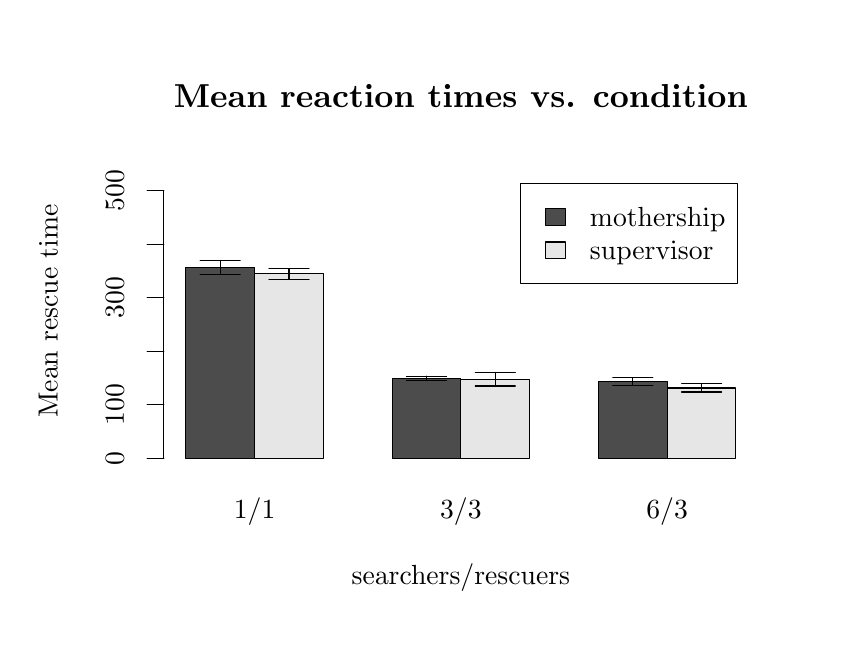
\begin{tikzpicture}[x=1pt,y=1pt]
\definecolor{fillColor}{RGB}{255,255,255}
\path[use as bounding box,fill=fillColor,fill opacity=0.00] (0,0) rectangle (289.08,216.81);
\begin{scope}
\path[clip] (  0.00,  0.00) rectangle (289.08,216.81);
\definecolor{drawColor}{RGB}{0,0,0}
\definecolor{fillColor}{gray}{0.30}

\path[draw=drawColor,line width= 0.4pt,line join=round,line cap=round,fill=fillColor] ( 57.15, 61.20) rectangle ( 82.00,130.17);
\definecolor{fillColor}{RGB}{230,230,230}

\path[draw=drawColor,line width= 0.4pt,line join=round,line cap=round,fill=fillColor] ( 82.00, 61.20) rectangle (106.85,127.84);
\definecolor{fillColor}{gray}{0.30}

\path[draw=drawColor,line width= 0.4pt,line join=round,line cap=round,fill=fillColor] (131.69, 61.20) rectangle (156.54, 90.09);
\definecolor{fillColor}{RGB}{230,230,230}

\path[draw=drawColor,line width= 0.4pt,line join=round,line cap=round,fill=fillColor] (156.54, 61.20) rectangle (181.39, 89.78);
\definecolor{fillColor}{gray}{0.30}

\path[draw=drawColor,line width= 0.4pt,line join=round,line cap=round,fill=fillColor] (206.23, 61.20) rectangle (231.08, 88.94);
\definecolor{fillColor}{RGB}{230,230,230}

\path[draw=drawColor,line width= 0.4pt,line join=round,line cap=round,fill=fillColor] (231.08, 61.20) rectangle (255.93, 86.62);
\end{scope}
\begin{scope}
\path[clip] (  0.00,  0.00) rectangle (289.08,216.81);
\definecolor{drawColor}{RGB}{0,0,0}

\node[text=drawColor,anchor=base,inner sep=0pt, outer sep=0pt, scale=  1.00] at ( 82.00, 39.60) {1/1};

\node[text=drawColor,anchor=base,inner sep=0pt, outer sep=0pt, scale=  1.00] at (156.54, 39.60) {3/3};

\node[text=drawColor,anchor=base,inner sep=0pt, outer sep=0pt, scale=  1.00] at (231.08, 39.60) {6/3};
\end{scope}
\begin{scope}
\path[clip] (  0.00,  0.00) rectangle (289.08,216.81);
\definecolor{drawColor}{RGB}{0,0,0}

\path[draw=drawColor,line width= 0.4pt,line join=round,line cap=round] (177.99,160.38) rectangle (256.65,124.38);
\definecolor{fillColor}{gray}{0.30}

\path[draw=drawColor,line width= 0.4pt,line join=round,line cap=round,fill=fillColor] (186.99,151.38) rectangle (194.19,145.38);
\definecolor{fillColor}{RGB}{230,230,230}

\path[draw=drawColor,line width= 0.4pt,line join=round,line cap=round,fill=fillColor] (186.99,139.38) rectangle (194.19,133.38);

\node[text=drawColor,anchor=base west,inner sep=0pt, outer sep=0pt, scale=  1.00] at (203.19,144.94) {mothership};

\node[text=drawColor,anchor=base west,inner sep=0pt, outer sep=0pt, scale=  1.00] at (203.19,132.94) {supervisor};

\node[text=drawColor,anchor=base,inner sep=0pt, outer sep=0pt, scale=  1.20] at (156.54,188.07) {\bfseries Mean reaction times vs. condition};

\node[text=drawColor,anchor=base,inner sep=0pt, outer sep=0pt, scale=  1.00] at (156.54, 15.60) {searchers/rescuers};

\node[text=drawColor,rotate= 90.00,anchor=base,inner sep=0pt, outer sep=0pt, scale=  1.00] at ( 10.80,114.41) {Mean rescue time};
\end{scope}
\begin{scope}
\path[clip] (  0.00,  0.00) rectangle (289.08,216.81);
\definecolor{drawColor}{RGB}{0,0,0}

\path[draw=drawColor,line width= 0.4pt,line join=round,line cap=round] ( 49.20, 61.20) -- ( 49.20,157.94);

\path[draw=drawColor,line width= 0.4pt,line join=round,line cap=round] ( 49.20, 61.20) -- ( 43.20, 61.20);

\path[draw=drawColor,line width= 0.4pt,line join=round,line cap=round] ( 49.20, 80.55) -- ( 43.20, 80.55);

\path[draw=drawColor,line width= 0.4pt,line join=round,line cap=round] ( 49.20, 99.89) -- ( 43.20, 99.89);

\path[draw=drawColor,line width= 0.4pt,line join=round,line cap=round] ( 49.20,119.24) -- ( 43.20,119.24);

\path[draw=drawColor,line width= 0.4pt,line join=round,line cap=round] ( 49.20,138.59) -- ( 43.20,138.59);

\path[draw=drawColor,line width= 0.4pt,line join=round,line cap=round] ( 49.20,157.94) -- ( 43.20,157.94);

\node[text=drawColor,rotate= 90.00,anchor=base,inner sep=0pt, outer sep=0pt, scale=  1.00] at ( 34.80, 61.20) {0};

\node[text=drawColor,rotate= 90.00,anchor=base,inner sep=0pt, outer sep=0pt, scale=  1.00] at ( 34.80, 80.55) {100};

\node[text=drawColor,rotate= 90.00,anchor=base,inner sep=0pt, outer sep=0pt, scale=  1.00] at ( 34.80,119.24) {300};

\node[text=drawColor,rotate= 90.00,anchor=base,inner sep=0pt, outer sep=0pt, scale=  1.00] at ( 34.80,157.94) {500};
\end{scope}
\begin{scope}
\path[clip] ( 49.20, 61.20) rectangle (263.88,167.61);
\definecolor{drawColor}{RGB}{0,0,0}

\path[draw=drawColor,line width= 0.4pt,line join=round,line cap=round] ( 69.57,127.60) -- ( 69.57,132.74);

\path[draw=drawColor,line width= 0.4pt,line join=round,line cap=round] ( 62.35,127.60) --
	( 69.57,127.60) --
	( 76.80,127.60);

\path[draw=drawColor,line width= 0.4pt,line join=round,line cap=round] ( 76.80,132.74) --
	( 69.57,132.74) --
	( 62.35,132.74);

\path[draw=drawColor,line width= 0.4pt,line join=round,line cap=round] ( 94.42,125.95) -- ( 94.42,129.73);

\path[draw=drawColor,line width= 0.4pt,line join=round,line cap=round] ( 87.19,125.95) --
	( 94.42,125.95) --
	(101.65,125.95);

\path[draw=drawColor,line width= 0.4pt,line join=round,line cap=round] (101.65,129.73) --
	( 94.42,129.73) --
	( 87.19,129.73);

\path[draw=drawColor,line width= 0.4pt,line join=round,line cap=round] (144.12, 89.26) -- (144.12, 90.91);

\path[draw=drawColor,line width= 0.4pt,line join=round,line cap=round] (136.89, 89.26) --
	(144.12, 89.26) --
	(151.34, 89.26);

\path[draw=drawColor,line width= 0.4pt,line join=round,line cap=round] (151.34, 90.91) --
	(144.12, 90.91) --
	(136.89, 90.91);

\path[draw=drawColor,line width= 0.4pt,line join=round,line cap=round] (168.96, 87.34) -- (168.96, 92.22);

\path[draw=drawColor,line width= 0.4pt,line join=round,line cap=round] (161.74, 87.34) --
	(168.96, 87.34) --
	(176.19, 87.34);

\path[draw=drawColor,line width= 0.4pt,line join=round,line cap=round] (176.19, 92.22) --
	(168.96, 92.22) --
	(161.74, 92.22);

\path[draw=drawColor,line width= 0.4pt,line join=round,line cap=round] (218.66, 87.65) -- (218.66, 90.24);

\path[draw=drawColor,line width= 0.4pt,line join=round,line cap=round] (211.43, 87.65) --
	(218.66, 87.65) --
	(225.89, 87.65);

\path[draw=drawColor,line width= 0.4pt,line join=round,line cap=round] (225.89, 90.24) --
	(218.66, 90.24) --
	(211.43, 90.24);

\path[draw=drawColor,line width= 0.4pt,line join=round,line cap=round] (243.51, 85.15) -- (243.51, 88.09);

\path[draw=drawColor,line width= 0.4pt,line join=round,line cap=round] (236.28, 85.15) --
	(243.51, 85.15) --
	(250.73, 85.15);

\path[draw=drawColor,line width= 0.4pt,line join=round,line cap=round] (250.73, 88.09) --
	(243.51, 88.09) --
	(236.28, 88.09);
\end{scope}
\end{tikzpicture}
